
\documentclass[xcolor=dvipsnames]{beamer}
\usepackage{tikz}
\usepackage{latexsym}
\usepackage{braket}
\usepackage{graphicx}
\usepackage{amsfonts}
\usepackage{amsmath}
\usepackage{verbatim}
\usepackage{amssymb}
\usepackage{amsthm}
\usepackage[english]{babel}
\usepackage[utf8]{inputenc}
\usepackage{listings}
\usepackage{color}
\usepackage{float}
\usepackage{geometry}
\usepackage{algorithm}
\usepackage{algpseudocode}
\usepackage{pdfpages}
\usetheme{default}
\usecolortheme[named=Brown]{structure} 
\setbeamertemplate{frametitle}[default][] 
\definecolor{lightbrown}{rgb}{0.933,0.890,0.773}

\setbeamerfont{section in head/foot}{size={\fontsize{8}{8}}}
\setbeamercolor{section in head/foot}{bg=lightbrown!5}
\setbeamercolor{head/foot}{ bg=Brown!45}
\setbeamercolor{frametitle}{fg=Brown, bg=lightbrown!30}
\setbeamercolor{block title}{bg=lightbrown}
\setbeamercolor{block body}{bg = lightbrown}
\setbeamertemplate{blocks}[rounded][shadow=true]


\setbeamertemplate{headline}{%
\leavevmode%
  \hbox{%
    \begin{beamercolorbox}[wd=\paperwidth,ht=3.5ex,dp=1.125ex, plus1fil]{palette quaternary}%
    \insertsectionnavigationhorizontal{\paperwidth}{}{\hskip 0cm}
    \end{beamercolorbox}%
  }
}

\makeatletter
    \newenvironment{withoutheadline}{
        \setbeamertemplate{headline}[default]
        \def\beamer@entrycode{\vspace*{-\headheight}}
    }{}
\makeatother


\logo{
\includegraphics[height=0.8cm]{unipi}\hspace{0.1cm}
\includegraphics[height=0.8cm]{anna}}
\setbeamertemplate{navigation symbols}{}


\title[framework]{
\includegraphics[height=1.3cm]{unipiinit2}
\includegraphics[width=0.5cm]{space}
\includegraphics[height=1.3cm]{annainit}\newline \newline
A Framework for static allocation of parallel OpenMP code on multi-core platforms\\}
\author[]{Giacomo Dabisias, Filippo Brizzi}
\institute[unipi]{
 Supervisors:
 E.Ruffaldi,
G. Buttazzo \\
\vspace*{1\baselineskip} 
  Universit\`a degli studi di Pisa,\\
  Scuola Superiore Sant'Anna\\
  Pisa,Italy\\[1ex]

 


}



\definecolor{blue}{RGB}{0,0,180}
\definecolor{darkblue}{RGB}{72,61,139} 
\definecolor{green}{rgb}{0,0.4,0}
\definecolor{gray}{rgb}{0.5,0.5,0.5}
\definecolor{darkgray}{rgb}{0.4,0.4,0.4}
\definecolor{mauve}{rgb}{0.58,0,0.82}
\definecolor{black}{rgb}{0,0,0}
\definecolor{purple}{RGB}{138,43,226}
\definecolor{ocra}{RGB}{218,165,32}
\definecolor{maroon}{rgb}{0.5,0,0}
\definecolor{darkgreen}{rgb}{0,0.5,0}
\definecolor{indianred}{RGB}{178,34,34}


\lstdefinelanguage{CCC}{ 
  breakatwhitespace=false,         
  breaklines=true,                 
  captionpos=b,                   
  frame=single,                    
  keepspaces=true,                 
  numbers=left,                    
  numbersep=5pt,                   
  numberstyle=\tiny\color{gray}, 
  rulecolor=\color{black},         
  showtabs=false,                  
  stepnumber=1,                    
  tabsize=2,                       
  title=\lstname,                   
  basicstyle=\scriptsize\tiny,
  stringstyle=\color{ocra},
  morestring=[b]",
  identifierstyle=\color{black},
  morecomment=[l][\color{maroon}]{pragma\ },
  morecomment=[l][\color{gray}]{//},
  morecomment=[s][\color{gray}]{/*}{*/},
  keywordstyle=[1]\color{blue},
  keywords=[1]{int,float,char, class, void, unsigned, struct, bool},
  keywordstyle=[0]\color{indianred},
  keywords=[0]{include,for,if,while,return,public,break}
}

\lstdefinelanguage{AST}{ 
  breakatwhitespace=false,         
  breaklines=true,                 
  captionpos=b,                   
  frame=single,                   
  keepspaces=true,                 
  rulecolor=\color{black},         
  showtabs=false,                  
  tabsize=2,                       
  title=\lstname,                   
  morekeywords={A}, 
  keywordstyle=\color{blue},
  language=C++,
  morecomment=[s][\color{gray}]{<}{>},
  stringstyle=\color{ocra},
 basicstyle=\color{black}\footnotesize\tiny
}



\date[February 2014]{February 28, 2014}

\begin{document}

\begin{withoutheadline}
\begin{frame}
  \titlepage
\end{frame}
\end{withoutheadline}

\begin{section}{Introduction}





\begin{frame}{\hskip 0.3cm Context and motivations}

Real-time systems are moving towards multicore architectures. The majority of multithread/core libraries target high performance systems. 

\begin{itemize}

\item Real-time applications need strict timing guarantees and predictability.

 \begin{center} Vs \end{center}

\item High performance systems try to achive a lower computation time in a best efford manner.

\end{itemize}

There is no actual automatic tool which has the advantages of HPC with timing contrains.

\end{frame}








\begin{frame}{\hskip 0.3cm Objectives}

The aim of this work is to create:

\begin{itemize}

\item An easy API to specify the concurrency between real- time tasks and scheduling parameters.

\item A way to visualize task concurrency and code structure as graphs.

\item A scheduling algorithm which supports multicore architectures, adapting to
the specific platform.

\item A run time support for the program execution which guarantees the scheduling order of tasks and their timing contrains.

\end{itemize}



\end{frame}











\begin{frame}{\hskip 0.3cm Design Choices: OpenMP and Clang}


OpenMP 

\begin{itemize}

\item Minimal code overhead.

\item Well spread standard.

\item Opensource and supported by several vendors like Intel and IBM.

\end{itemize}

Clang

\begin{itemize}

\item Provides code analysis and source to source translation capabilities.

\item Modularity and great efficency.

\item Opensource and supported by several vendors like Google and Apple.

\end{itemize}
In July 2013 Intel released a patched version of Clang which fully supports the OpenMP 3.3 standard. 

\end{frame}











\begin{frame}{\hskip 0.3cm General Design}

The framework takes as input a C++ code annotated with OpenMP.

\begin{itemize}

\item The pragmas are extracted with all relevant informations using Clang and saved as XML .

\item The input code is rewritten to perform profiling .

\item The scheduler tool uses these informations to create a possible schedule.

\item The input code is rewritten to allow execution according to the generated schedule.

\item The code is then executed with a custom run-time support.

\end{itemize}

\end{frame}











\begin{frame}{\hskip 0.3cm }

\begin{tikzpicture}[remember picture,overlay]
            \node[at=(current page.center)] {
                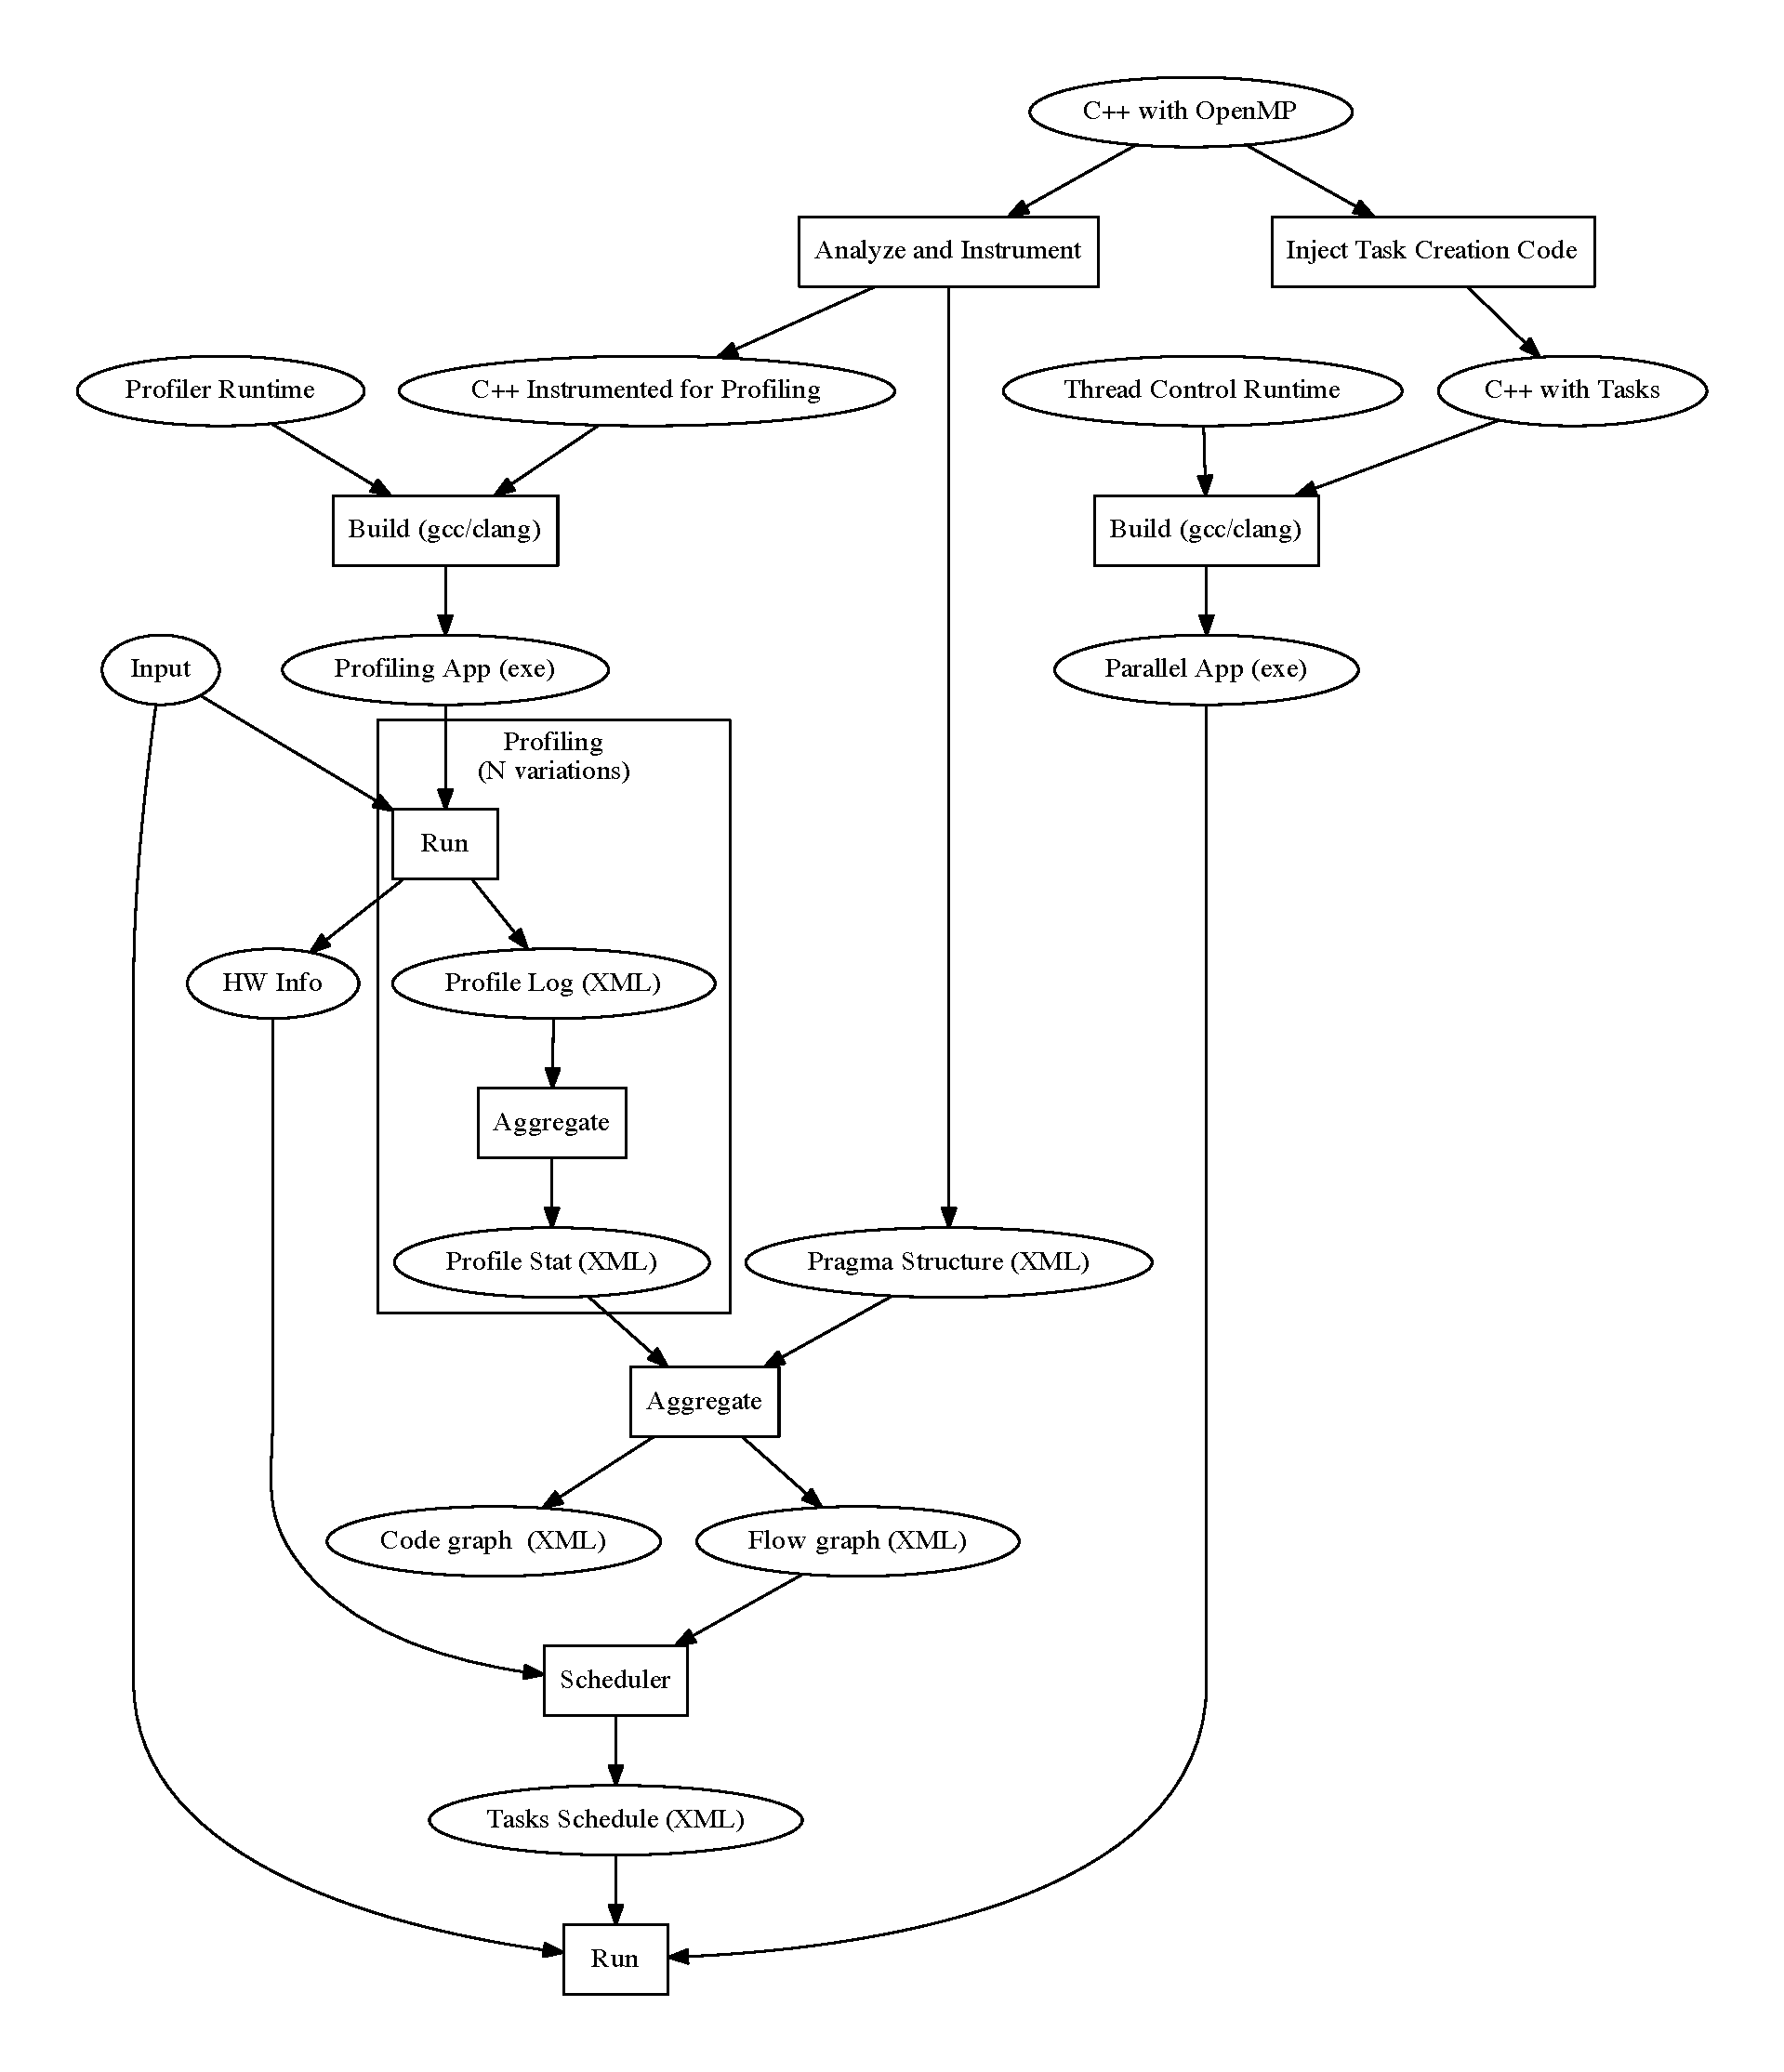
\includegraphics[scale = 0.25]{framework.pdf}
            };
        \end{tikzpicture}

\end{frame}









\begin{frame}{\hskip 0.3cm Graphs}


The framework creates three types of graphs to visualize and work on the extracted data 


\begin{itemize}		

\item Code Graph: represents the nested structure of the pragmas in the source code.

\item Flow Graph: represents the parallel execution flow and the synchronization barriers.

\item Agumented Flow Graph: enhances the Flow Graph with the profiling informations and the function calls.

\item Schedule graph: enhances the Agumented Flow Graph with scheduling informations.


\end{itemize}			

The graphs are stored using Python objects and visualized using Graphviz.



\end{frame}








\begin{frame}{\hskip 0.3cm OpenMP }

Multiple threads of execution perform tasks defined by directives.

\begin{itemize}
\item Each directive applies to  a block of C++ code embedded in a scope.

\item Allows nested parallelism though nested directives.

\item Clauses allow variables management.
\end{itemize}

\begin{block}

$\#$pragma omp directive-name [clause[ [,] clause]...] new-line

\end{block}

Choosen subset for the framwork:

\begin{itemize}

\item Control directives : parallel, sections, single.

\item Working directives : task, section, for.

\end{itemize}

\end{frame}












\begin{frame}{\hskip 0.3cm OpenMP}

\begin{figure}
\centering
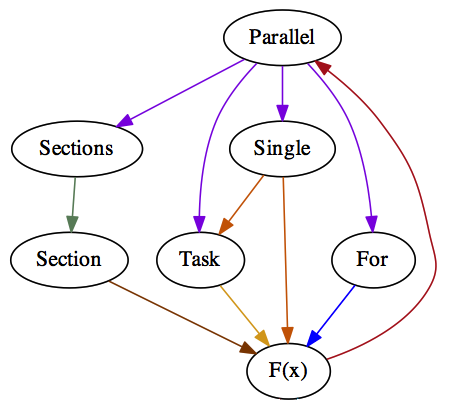
\includegraphics[scale = 0.45]{ompstructure}

\end{figure}

\end{frame}


\begin{frame}[fragile]{\hskip 0.3cm Simple Example}

\begin{columns}

\begin{column}{5cm}
\begin{lstlisting}[language=CCC]
void work(int bar){
    #pragma omp parallel for
    for (int i = 0; i < bar; ++i)
    {
       //do stuff
    }  
};
int main(int argc, char* argv[]) {
    int bar;
    #pragma omp parallel private(bar)
    {
        #pragma omp sections
        {
            #pragma omp section
            {   
                //do stuff (bar)
                work(bar);
            }
            #pragma omp section
            {
                //do stuff (bar)
                work(bar);
            }
        }
    }
}
\end{lstlisting}

\end{column}

\begin{column}{6.5cm}
\vskip -1cm
\begin{figure}

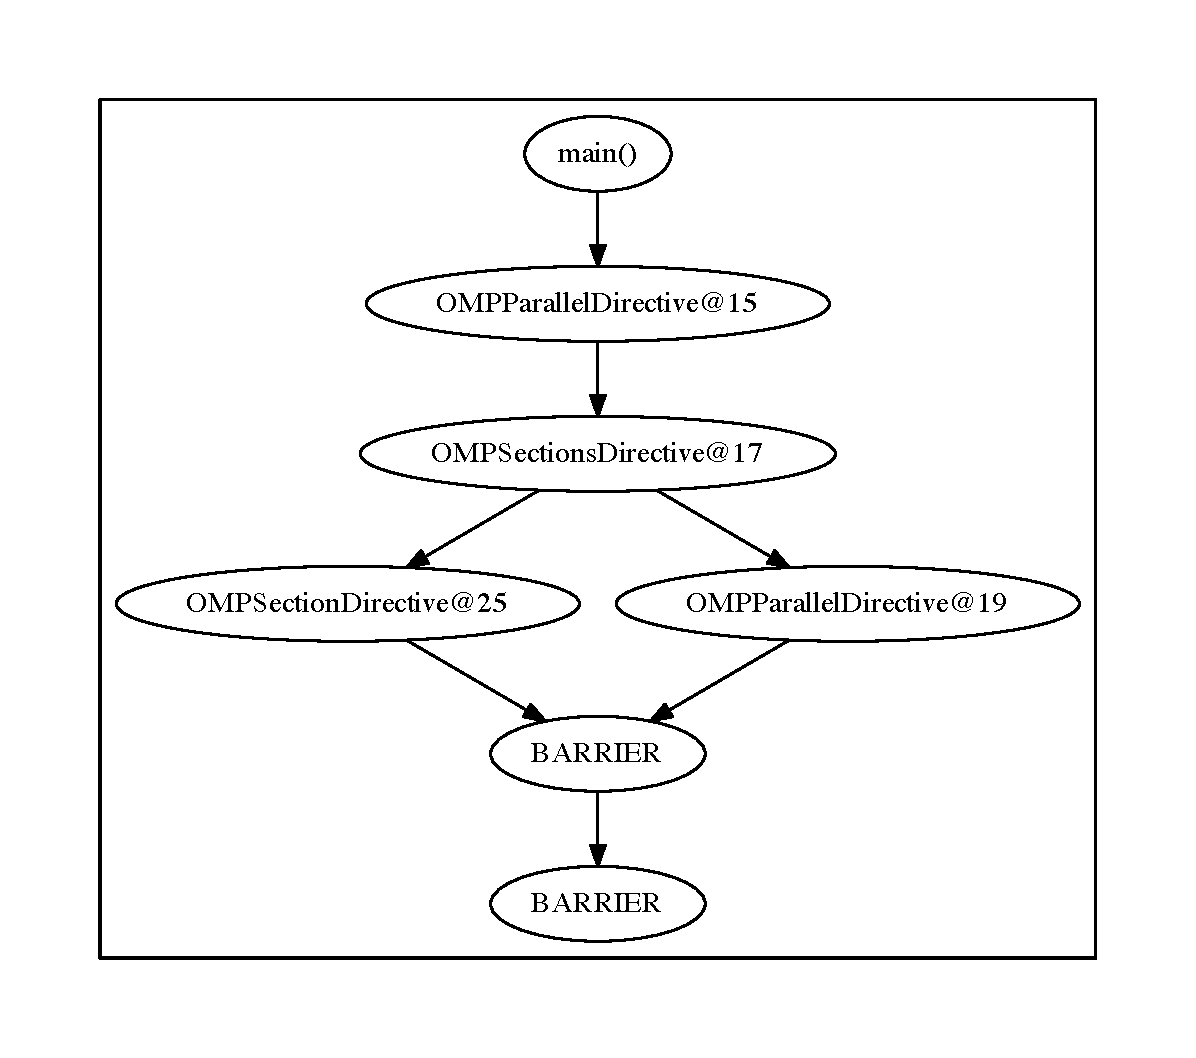
\includegraphics[scale=0.3]{main.pdf}
\end{figure}
\vskip -1.5cm
\begin{figure}
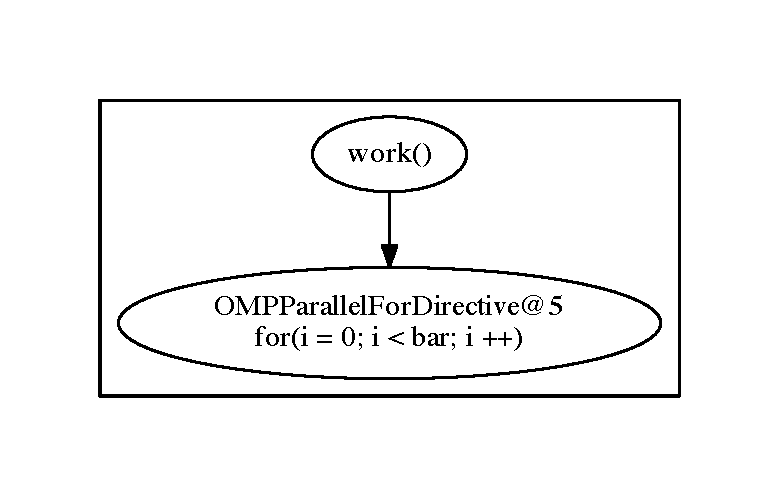
\includegraphics[scale=0.3]{work.pdf}
\end{figure}

\end{column}

\end{columns}

\end{frame}















\begin{frame}{\hskip 0.3cm Clang}

Clang and OpenMP:

The strength of Clang lies in its implementation of the Abstract Syntax Tree (AST).
\begin{itemize}

\item Closely resembles both the written C++ code and the C++ standard.

\item Clang’s AST nodes are modeled on a class hierarchy that does not have a common ancestor.

\item Hundreds of classes for a total of more than one hundred thousand lines of code.

\end{itemize}
\end{frame}
















\begin{frame}{\hskip 0.3cm Clang - AST}

To traverse the AST, Clang provides the RecursiveASTVisitor class.
\begin{itemize}

\item Very powerful and easy to learn interface

\item Possibility to create a custom visitor that triggers only on specific nodes.


\end{itemize}

Clang supports the insertion of custom code through the Rewriter class.
\begin{itemize}

\item Allows insertion, deletion and replacement of code.

\item Operations are performed during the AST visit.

\item A new source file with all the modifications is generated at the end of the visit.

\end{itemize}

\end{frame}














\begin{frame}[fragile]{\hskip 0.3cm Clang - AST}

\begin{columns}

\begin{column}{4cm}
\begin{lstlisting}[language=CCC]
class A {
public:
  int x;
  void set_x(int val) {
       x = val * 2;
  }	
  int get_x() {
      return x;
  }
};
int main() {
    A a;
    int  val = 5;
    a.set_x(val);
}
\end{lstlisting}
\end{column}

\begin{column}{7.3cm}

\begin{lstlisting}[language=AST]
TranslationUnitDecl
|-CXXRecordDecl <clang_ast_test.cpp:2:1, line:13:1> class A
| |-CXXRecordDecl <line:2:1, col:7> class A
| |-AccessSpecDecl <line:3:1, col:7> public
| |-FieldDecl <line:4:2, col:6> x 'int'
| |-CXXMethodDecl <line:5:2, line:7:2> set_x 'void (int)'
| | |-ParmVarDecl <line:5:13, col:17> val 'int'
| | `-CompoundStmt <col:22, line:7:2>
| |   `-BinaryOperator <line:6:3, col:13> 'int' lvalue '='
| |     |-MemberExpr <col:3> 'int' lvalue ->x
| |     | `-CXXThisExpr <col:3> 'class A *' this
| |     `-BinaryOperator <col:7, col:13> 'int' '*'
| |       |-ImplicitCastExpr <col:7> 'int' <LValueToRValue>
| |       | `-DeclRefExpr <col:7> 'int' lvalue ParmVar 'val' 'int'
| |       `-IntegerLiteral <col:13> 'int' 2
...
\end{lstlisting}
\end{column}

\end{columns}


\end{frame}








\end{section}
\begin{section}{Framework}














\begin{frame}[fragile]{\hskip 0.3cm Instrumentation for Profile}

\begin{itemize}
\item Creation of a custom profiler to time pragma code blocks and functions.  No existing profiling tool allows this operation.

\begin{itemize}

\item Code is instrumented with calls to a custom run-time support.

\item Extracted information: execution time, children execution time, caller identifier, for loop counter.

\item Output is saved in an XML file.

\end{itemize}
\end{itemize}
\begin{lstlisting}[language=CCC]
...
//#pragma omp parallel for
if( ProfileTracker profile_tracker = ProfileTrackParams(3, 5, bar - 0))
	for (int i = 0; i < bar; ++i)
	{
    		//do stuff
	}
...
//#pragma omp section
if( ProfileTracker profile_tracker = ProfileTrackParams(12, 25))
{
    //do stuff (bar)
    work(bar);
}
...
\end{lstlisting}

\end{frame}












\begin{frame}{\hskip 0.3cm Profile}

\begin{columns}

\begin{column}{5cm}
\begin{itemize}

\item The profiled code is executed $N$ times and statistics are obtained. 

\item It is possible to use different arguments for the execution.

\item An edge is added for each function call that contains pragmas.

\end{itemize}
\end{column}

\begin{column}{7.5cm}
\vskip -0.5cm
\begin{figure}
\centering
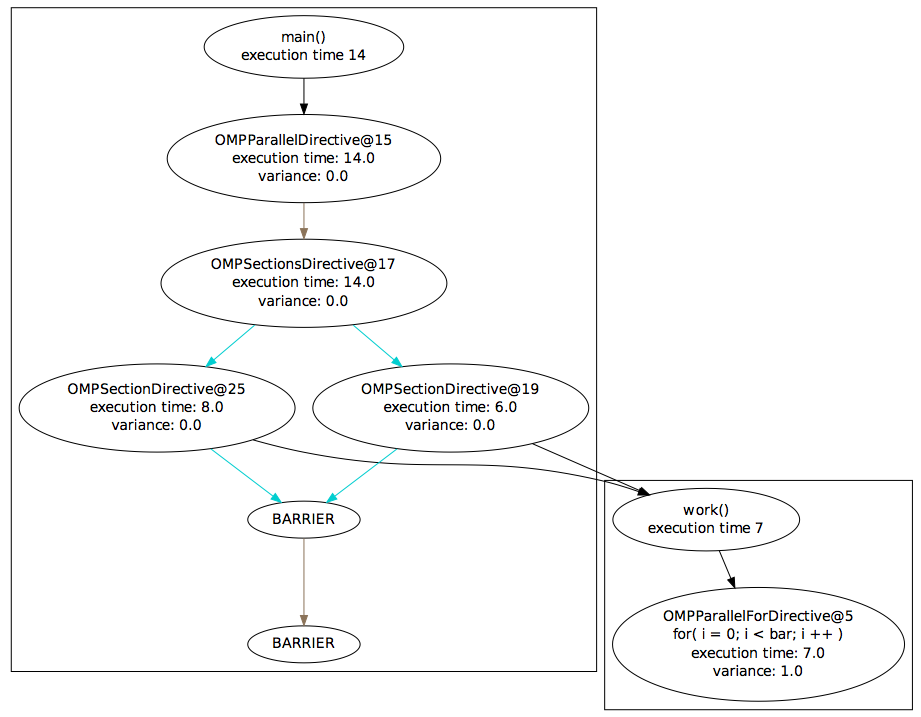
\includegraphics[scale=0.22]{call_graph.png}

\end{figure}
\end{column}

\end{columns}

Possible evolution: probabilistic analysis of the function calls and execution times.


\end{frame}








\begin{frame}{\hskip 0.3cm Scheduler }

The scheduler takes as input the Agumented Flow Graph and the program's deadline.

\begin{itemize}

\item Since the problem is $NP$-complete, all possible schedules have to be checked.

\item It is possible to set a fixed amount of computation time.

\item A parallel version of the scheduler has been developed which achieves better results in a fixed amount of time.

\end{itemize}

The final schedule is saved as XML file which specifies for each pragma the thread identifier.

\end{frame}







\begin{frame}{\hskip 0.3cm Scheduler - Algorithm}
\vskip -0.9cm
\begin{columns}

\begin{column}{6cm}

The scheduler assigns each task to a flow using a search tree. Each flow will be allocated to a different thread.

\end{column}

\begin{column}{4.5cm}

\begin{figure}
\centering
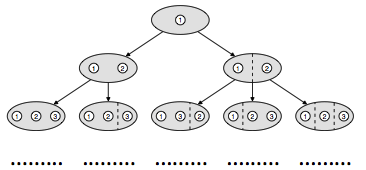
\includegraphics[scale=0.37]{search_tree.png}
\end{figure}
\end{column}


\end{columns}

\begin{itemize}

\item All tasks are stored in an unordered list.

\item The scheduler extracts one task at a time adding it to the current flows and to a new flow.

\item The algorithm splits each pragma for node.

\item The scheduler recurs on each flow pruning it as soon as possible.

\item When a leaf is reached, the algorithm checks if the current solution is better then the previous one.

\end{itemize}

\end{frame}












\begin{frame}{\hskip 0.3cm Scheduler - Feasibility}

The produced schedule does not account for precedence relations. A modified version of Chetto\&Chetto (1990) has been used to check the feasibility.

\begin{itemize}

\item All deadlines are set for each task starting from the last one.

\item All arrival times are set for each task starting from the first and accounting for precedence relations.

\item If all deadline are positive and each arrival time is less then the corresponding deadline the schedule is produced.

\end{itemize}



\end{frame}













\begin{frame}{\hskip 0.3cm Final Execution - Instrumentation}

Each pragma block is transformed in a custom task.


\begin{itemize}

\item Each pragma code block is embedded in a function call.

\item The function is member of a class defined inside the scope of the pragma block.

\item All the variables used in the pragma block, but declared outside are passed to the class's constructor.

\item The nested pragma structure is not changed.

\item Each for is rewritten in order to allow it to be splitted.

\end{itemize}





\end{frame}













\begin{frame}[fragile]{\hskip 0.3cm Final Execution - Instrumentation Example}

\begin{lstlisting}[language=CCC]
 //#pragma omp section
{
    class Nested : public NestedBase {
    public: 
        virtual shared_ptr<NestedBase> clone() const { 
          return make_shared<Nested>(*this); 
        } 
        Nested(int pragma_id, int & bar) : 
            NestedBase(pragma_id), bar_(bar) {}
        int & bar_;
            
        void fx(int & bar){   
            //do stuff (bar)
            work(bar);
            launch_todo_job(); 
        }
        void callme() {
            fx(bar_);
        }
    };
    shared_ptr<NestedBase> nested_b = make_shared<Nested>(19, bar);                             
    if(ThreadPool::getInstance()->call(nested_b)) 
        todo_job_.push(nested_b); 
}
\end{lstlisting}


\end{frame}








\begin{frame}{\hskip 0.3cm Final Execution - Run-time }

The run-time parses the generated XML schedule. 

\begin{itemize}

\item Instantiates all the requested threads using the standard thread library.

\item Creates a work queue for each thread.

\item When invoked it receives a task and extracts from the schedule the designated execution thread.

\item The task is enhanced with synchronization variables.

\item The task is pushed in the corresponding working  thread queue.

\end{itemize}

\end{frame}












\begin{frame}{\hskip 0.3cm Final Execution - Runt-time}

Each thread behaves as follows

\begin{itemize}

\item An infinite loop is executed polling the its work queue.

\item After work completion all the necessary synchronizations are perfomed before continuing with the next task.

\end{itemize}

\begin{figure}
\centering
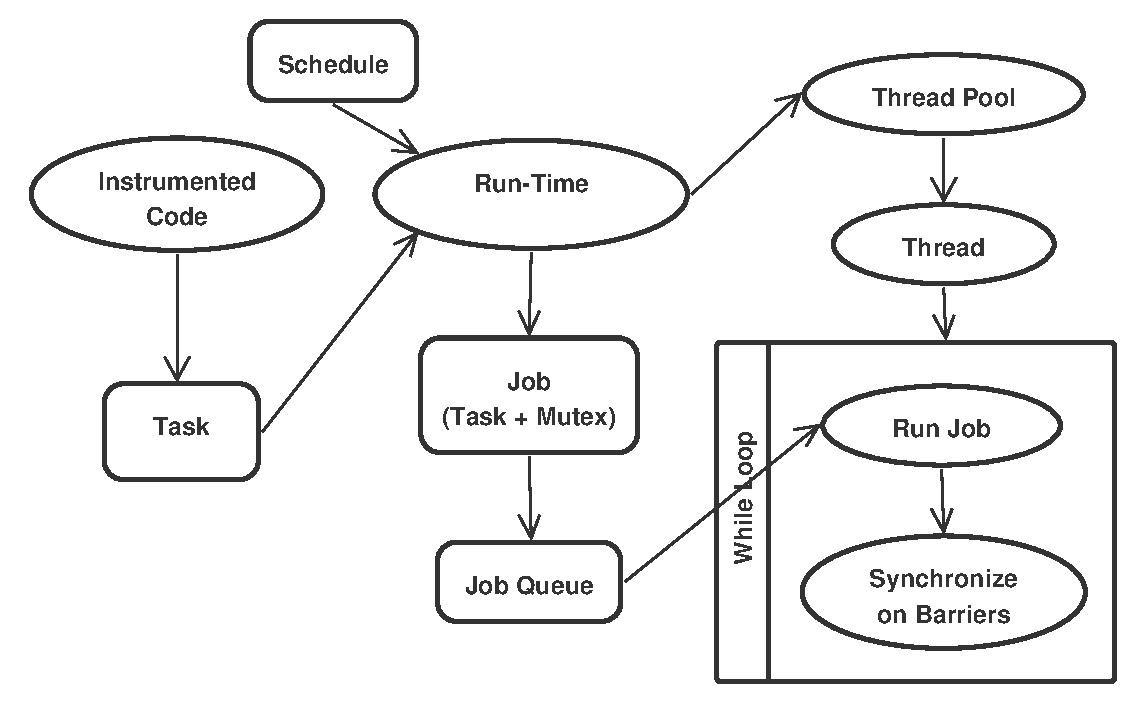
\includegraphics[scale=0.40]{runtime_execution.pdf}
\end{figure}




\end{frame}











\end{section}
\begin{section}{Test}











\begin{frame}{\hskip 0.3cm General structure}

Face recognition algorithm in OpenCV.

\begin{itemize}

\item Takes as input two videos to simulate the human view.

\item Frames are dispatched in blocks of $N$ frames.
 
\item All faces are detected and circled in each frame.

\item All frames are saved on disk.


\end{itemize}

Three different qualities of the same videos have been used to test the algorithm (480p, 720p, 1080p).


\end{frame}
















\begin{frame}{\hskip 0.3cm General structure}

\vskip -1cm

\begin{figure}
\hskip -1cm

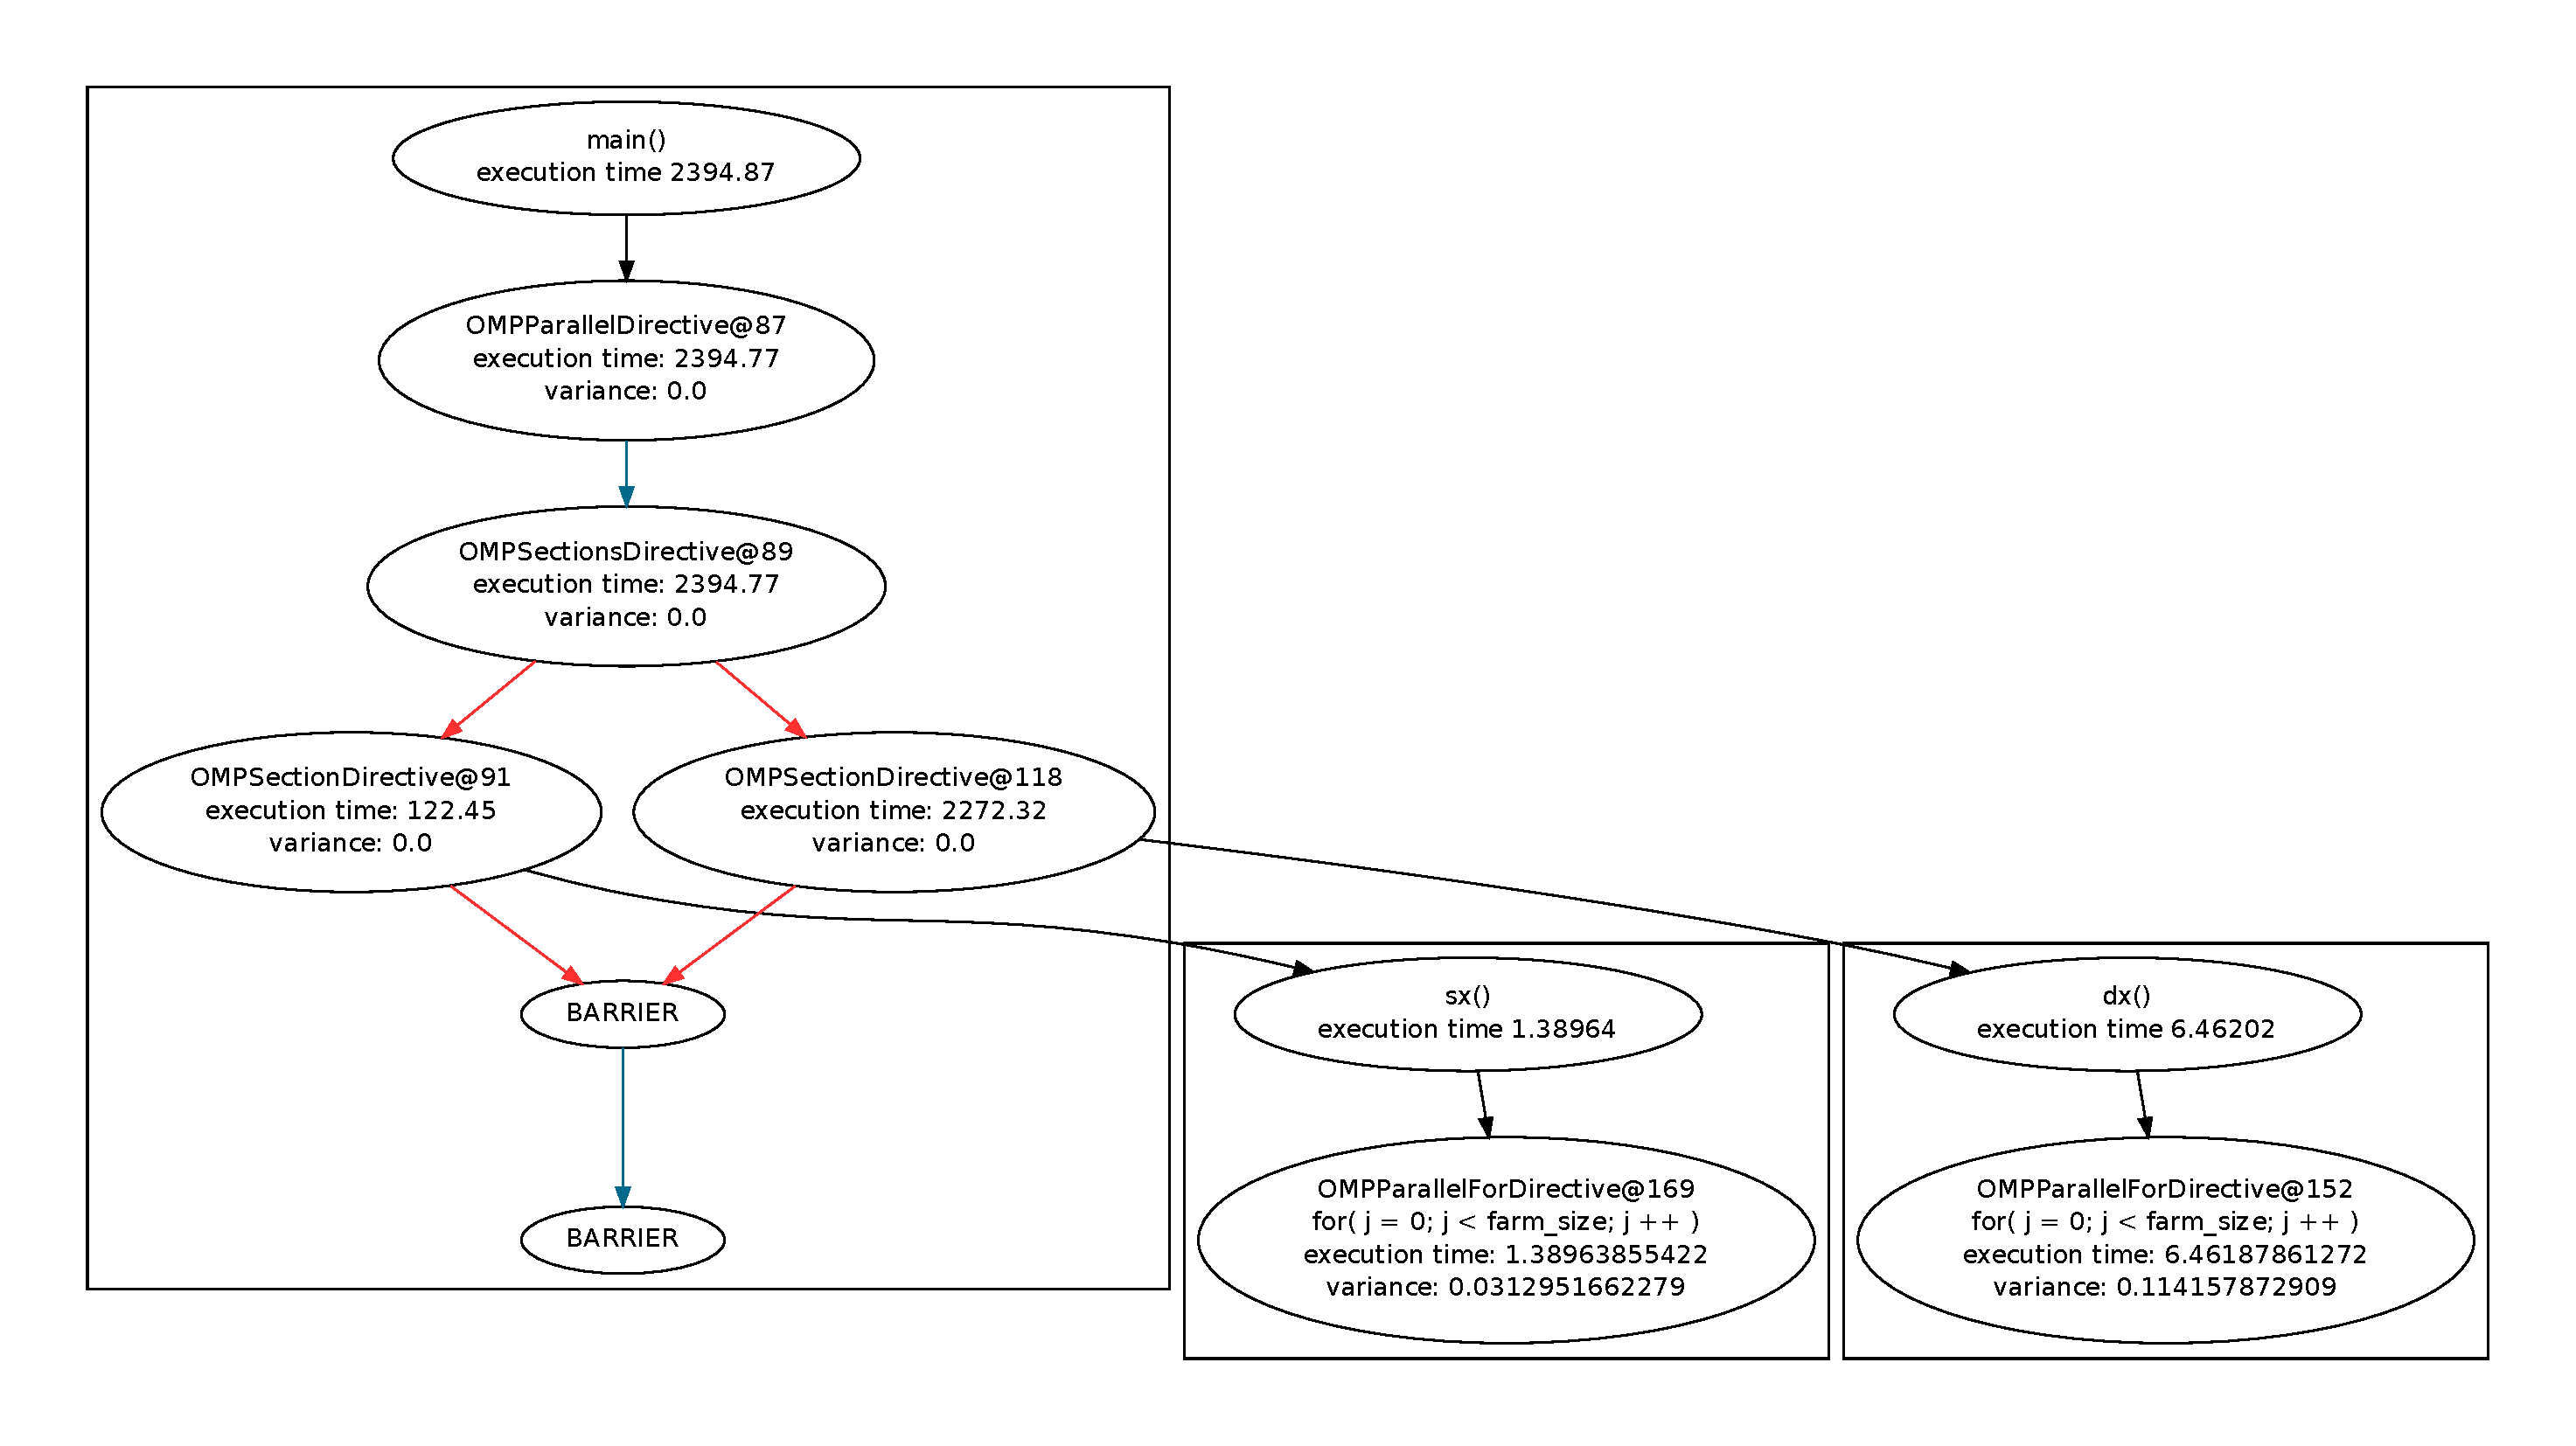
\includegraphics[scale=0.23]{test.pdf}
\end{figure}

\end{frame}

















\begin{frame}{\hskip 0.3cm Results}
\vskip -1cm
\begin{itemize}

\item 6 cores with hyperthreading.

\item Statistics are calculated over 5 executions.

\end{itemize}


\begin{center}
\resizebox{\linewidth}{!}{

\begin{tabular}{| l || c || c | c || c | c |}
\hline
 & \multicolumn{1}{|c||}{Sequential} & \multicolumn{2}{|c||}{OpenMP} & \multicolumn{2}{|c|}{Soma} \\
\cline{2-6}
  & $T_{seq}[s]$ & $T_c(n)[s]$ & $\epsilon (n) = \frac{T_{seq}}{nT_c(n)}$ & $T_c(n)[s]$ & $\epsilon (n) = \frac{T_{seq}}{nT_c(n)}$ \\
\cline{2-6}
\hline
480p(4) & 750 & 195 & 0.96 & 195 & 0.96 \\
\hline
720p(4) & 3525 & 921 & 0.96 & 921 & 0.96 \\
\hline
1080p(4) & 8645 & 2271 & 0.95 & 2270 & 0.95 \\
\hline 
\hline
480p(6) & - & 133 & 0.94 & 134 & 0.93 \\
\hline
720p(6) & - & 627 & 0.94 & 629 & 0.93 \\
\hline
1080p(6) & - & 1536 & 0.94 & 1539 & 0.94 \\
\hline 
\hline
480p(12) & - & 98 & 0.64 & 92 & 0.68 \\
\hline
720p(12) & - & 427 & 0.69 & 426 & 0.69 \\
\hline
1080p(12) & - & 1043 & 0.69 & 1035 & 0.70 \\
\hline 
\end{tabular} }
\end{center}

\end{frame}












\begin{frame}{\hskip 0.3cm Results - Service Time}

Service time in second of each thread (gap between the delivery of a parsed image).

\begin{itemize}

\item Soma variance $<$ OpenMP variance

\item Video quality 720p, 6 cores. 

\end{itemize}

\begin{center}
\resizebox{\linewidth}{!}{

\begin{tabular}{| l || c | c || c | c || c | c |} 
\hline
  Thread & \multicolumn{2}{|c||}{Sequential} & \multicolumn{2}{|c||}{OpenMP} & \multicolumn{2}{|c|}{Soma} \\
\cline{2-7}
& $T_s$ & $variance$ & $T_s$ & $variance$ & $T_s$ & $variance$ \\
\cline{2-7}
\hline
0 & 1.3263 & 0.1968 & 1.4226 & 0.0092 & 1.4987 & 0.0065  \\
\hline
1 & - & - & 1.4225 & 0.0090 & 1.4297 & 0.0065 \\
\hline
2 & - & - & 1.4225 & 0.0098 & 1.4298 & 0.0065 \\
\hline 
3 & - & - & 1.4257 & 0.0125 & 1.4117 & 0.0067 \\
\hline
4 & - & - & 1.4256 & 0.0129 & 1.4111 & 0.0060 \\
\hline
5 & - & - & 1.4256 & 0.0129 & 1.4117 & 0.0060  \\
\hline
\end{tabular}}
\end{center}

Performances remain consistent changing the video quality.








\end{frame}












\begin{frame}{\hskip 0.3cm Results - Mean Service Time}

\begin{center}
\resizebox{\linewidth}{!}{

\begin{tabular}{| l || c || c | c || c | c |}
\hline
 & \multicolumn{1}{|c||}{Sequential} & \multicolumn{2}{|c||}{OpenMP} & \multicolumn{2}{|c|}{Soma} \\
\cline{2-6}
  & $mean\ T_s$ & $mean\ T_s$ & $mean\ var$ & $mean\ T_s$ & $mean\ var$ \\
\cline{2-6}
\hline
480p(4) & 750 & 195 & 0.96 & 195 & 0.96 \\
\hline
720p(4) & 3525 & 921 & 0.96 & 921 & 0.96 \\
\hline
1080p(4) & 8645 & 2271 & 0.95 & 2270 & 0.95 \\
\hline 
\hline
480p(6) & - & 133 & 0.94 & 134 & 0.93 \\
\hline
720p(6) & - & 627 & 0.94 & 629 & 0.93 \\
\hline
1080p(6) & - & 1536 & 0.94 & 1539 & 0.94 \\
\hline 
\hline
480p(12) & - & 98 & 0.64 & 92 & 0.68 \\
\hline
720p(12) & - & 427 & 0.69 & 426 & 0.69 \\
\hline
1080p(12) & - & 1043 & 0.69 & 1035 & 0.70 \\
\hline 
\end{tabular} }
\end{center}







\end{frame}













\begin{frame}{\hskip 0.3cm Results - (Jitter)}
\end{frame}












\begin{frame}{\hskip 0.3cm Results - Comments}
\end{frame}












\end{section}
\begin{section}{Conclusion and Future Directions}












\begin{frame}{\hskip 0.3cm }
\end{frame}












\end{section}

\end{document}
